% Source: graduate-coursework/Prior_Semesters/Fa23/ELCT432/exercises/PA3_DSB_SC_Modulation.tex

\documentclass[border=4pt]{standalone}
\usepackage{amsmath}
\usepackage{graphicx}
\usepackage{tikz}
\usetikzlibrary{arrows,shapes,positioning}

\begin{document}
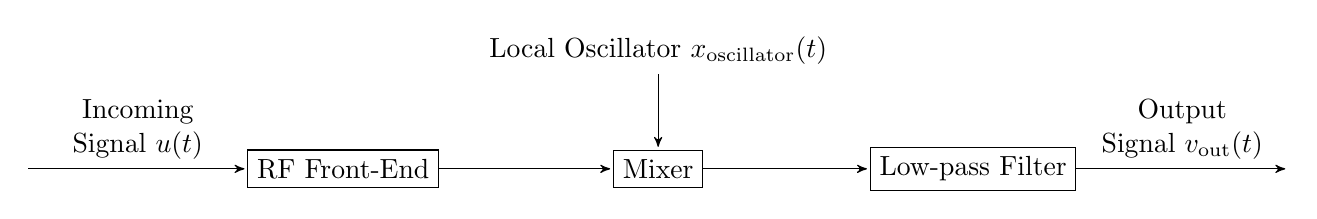
\begin{tikzpicture}[>=stealth',shorten >=1pt,auto,node distance=4cm,
                    block/.style={rectangle, draw, align=center}]
  % Nodes
  \node[block] (rf) {RF Front-End};
  \node[block, right of=rf] (mixer) {Mixer};
  \node[block, right of=mixer] (lpf) {Low-pass Filter};
  \node[coordinate, left of=rf] (input) {};
  \node[coordinate, right of=lpf] (output) {};

  % Edges
  \draw[->] (input) -- node[name=u, align=center] {Incoming\\Signal \(u(t)\)} (rf);
  \draw[->] (rf) -- node[name=v, align=center] {} (mixer);
  \draw[->] (mixer) -- node[name=w, align=center] {} (lpf);
  \draw[->] (lpf) -- node[name=x, align=center] {Output\\Signal \(v_{\text{out}}(t)\)} (output);

  % Labels
  \node[above of=mixer, node distance=1.5cm] (lo) {Local Oscillator \(x_{\text{oscillator}}(t)\)};
  \draw[->] (lo) -- (mixer);
\end{tikzpicture}
\end{document}
